\section{Concrete approaches}\label{approaches}
\subsection{Narratology excursion}
The following two subsections (\ref{fabula} and \ref{discourse}) will showcase two concrete cases of story telling by application of AI planning. Because they approach the subject matter on different levels a distiction is required. It will be necessary to distinguish between \emph{fabula} (or \emph{story}) on the one hand, and \emph{discourse} (or \emph{plot}) on the other hand.\\
Chatman writes in \cite{Chatman1980} (furthermore cited in \cite{Herman10}):
\begin{quote}
''In simple terms, the story is the \emph{what} in a narrative that is depicted, discourse is the \emph{how}.''

(Note: Since \emph{story} and \emph{plot} are more commonly used in everyday language and might lead to confusion or wrong assumptions the remainder of this document will refer to the two concepts as \emph{fabula} and \emph{discourse}.)
\end{quote}
To illustrate the difference with an example: viewers of a movie might be presented with a character A, talking about what a character B has done (assume A's report to be truthful and B's action to be relevant for the movie). On the level of the fabula (the narrative structure), we have B doing something. On the level of the discourse (how this is conveyed to the recipient) we have A talking about it. When watching a movie or reading a book one is presented with a discourse and automatically constructs a fabula in their head.
% - 2 approaches address story/narrative at different levels
% - fabula vs discourse
\subsection{Planning a fabula}\label{fabula}
In \cite{Haslum14} Haslum shows how a specific model of story generation proposed for the IPOCL planner\cite{Riedl10} can be compiled into a classic planning problem. The model in question is designed to create fabulae and incorporates the notion of character intetions. The following subsection will describe the story world modeling in general. After that aforementioned compilation will be adressed.

\subsubsection{Story world modeling}
The central building blocks in this apporach are story characters for which certain abilities are defined. For illustration purposes a story world which is loosely based on the tale of Aladdin is used. Characters are humans (Aladdin, Jasmine, king Jafar) and monsters (a genie, a dragon). The characters' abilities are actions which can be divided into intentional actions and happenings. The former are deliberate interactions with the story world or other characters (such as traveling between locations or slaying a monster) while the latter are unintentional effects (e.g. a monster scaring a human because of its appearance or a human falling in love with another).

In order to create coherent, believable fabulae the modeling lays its focus on intentionality. Apart from the desired story outcome (the goal of the overall planning problem) characters can have their own goals which can arise and change through influence by the story world. Intentionality can also be caused by delegation --- i.e. a character $A$ evokes a character goal in another character $B$ (for example through a command or persuasion). Most importantly character goals allow for \emph{intentional plans} which characters can pursue. When a character has a goal and carries out an action in order to reach it, the action is said to be performed in a \emph{frame of commitment}. Formally these terms are defined as follows:
\begin{quote}
''\textbf{Definition 1} An intentional plan is one in which every occurrence of an intentional action is part of some frame of commitment. A frame of commitment is a subset $S'$ of steps (i.e., action occurrences) in the plan, associated with a modal literal $(intends\ A\ g)$, satisfying four requirements: (1) Character $A$ is an actor of every step in $S'$. (2) There is a final step $s_{fin}\in S'$ that makes $g$ true. (3) There is a motivating step $s_m$ in the plan, which adds $(intends\ A\ g)$ and which precedes all steps in $S'$. We’ll say there is a motivational link from $s_m$ to every step in the frame of commitment, $S'$. Note that $s_m$ is not part of $S'$. (4) From each step in $S'$ other than $s_{fin}$ there is a path of causal or motivational links to $s_{fin}$. A complete (fabula) plan is one that is both intentional and valid in the classical sense.'' \cite{Haslum14}
\end{quote}
To visually aid the formal definition consider figure \ref{fig:intplan} on page \pageref{fig:intplan}. Arrows are to represent actions and dashed lines an arbitrary sequence of actions not shown. If all blue arrows are actions carried out by character $A$ then the frame of commitment is $S'=\{s_i,s_{i+1},s_{i+x},s_{fin}\}$. Note that $s_m$ does not necessarily have to be an action of $A$ since intention can be delegated and that the intentional plan which includes $S'$ may contain an arbitrary number of happenings unrelated to $S'$ or $g$.
\begin{figure}[htbp]
 \centering
 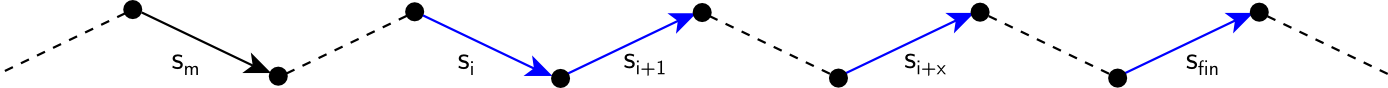
\includegraphics[scale=0.8]{intentional_plan}
 \caption{Visual example of a frame of commitment.}
 \label{fig:intplan}
\end{figure}

Ensuring that character goals are pursued by means of intentional plans is referred to as \emph{explicit justification tracking}. In \cite{Riedl10} this is performed by the IPOCL planner but in \cite{Haslum14} it is incorporated into the planning problem. This is accomplished by the main compilation described in \cite{Haslum14} and will be briefly discussed in the following subsection.

% - (desired) story outcome
% - character goals (can change, are influenced by other characters / events)
% - intentional agents (actions percievable as contributing to goals)
% - characters (humans, monsters (genie, dragon))
%     - have given abilities (travel betw. locations, slay monsters, take things from dead, gain control over (genie), fall in love, marry)
%     -> move in world, interact w/ other chars + world/objects
% - intentional actions vs. happenings (e.g. monster frightens human, human falls in love)
% - delegating actions (command, persuade, bribe, ... other char to so sth.)
% - intentional plan
%     -> frame of commitment
% - 
% - 
\subsubsection{Compilation}
The original story generation model includes modal literals in the form of $(intends\ A\ g)$ in order to handle intentionality. For the compilation into a classic planning problem predicates are introduced for intention, delegation and justification. Intention literals are used as preconditions for intentional actions, which allows the modeling of frames of commitment --- e.g. $(intends\h dead\ Aladdin\ Dragon)$ as a precondition for every action in Aladdins frame of commitment to slay the dragon including the $s_{fin}$ of him achieving his goal. Delegation and justification literals, on the other hand, are used for justification tracking. They are true in the initial state, required to be true at the goal, made false by certain intentional actions and then set up in a way such that only if motivational link as described in Definition 1 are adhered to will they become true again.

Description and discussion of this compilation's precise nature take up most of \cite{Haslum14} and can therefore not be covered here. To get an intuition of a possible output consider below example of a monster slaying action in PPDL-like syntax.
\begin{lstlisting}[frame=single,basicstyle=\scriptsize,numbers=left,numberstyle=\tiny]
(:action slay-1-because-intends-dead
    :parameters (?knight - knight ?monster - monster ?where - place)
    :precondition (and (alive ?knight) (at ?knight ?where)
                       (alive ?monster) (at ?monster ?where)
                       (intends ?knight (dead ?monster))
                  (not (exists (?c) (and (not (= ?c ?knight))
                                         (delegated ?c (dead ?monster))))))
    :effect (and (not (alive ?monster)) (dead ?monster)
        (justified (at ?knight ?where) (intends ?knight (dead ?monster)))
        (justified (at ?monster ?where) (intends ?knight (dead ?monster)))
        (not (delegated ?knight (dead ?monster)))))
\end{lstlisting}
A notable restriction of the compilation is that a delegated goal can only be achieved by the character it has been delegated to. In case of above monster slaying example this can be seen in lines 6 and 7. The monster may only be slain if there exists no other knight to whom the death of the monster has already been delegated.
\subsubsection{Result}
As already mentioned the story generation model at hand is designed to create fabulae. The result a planner produces therefore is a story \emph{structure}. (TODO: Fig. 1 from Haslum paper in appendix or just mention?)

% - modal literals intends, delegated, justified (in compilation expressed as modal predicates
% - intentions are preconditions of intentional actions
% - no actions can be taken that delegate or achieve a goal that is already delegated to another character
% - 
\subsection{Planning a discourse}\label{discourse}
In \cite{Porteous10} Porteous, Cavazza, and Charles\\
figure \ref{fig:modproc} on page \pageref{fig:modproc}
\subsubsection{Story world modeling}
% - narrative control knowlege
% - PoV
\begin{figure}[htbp]
 \centering
 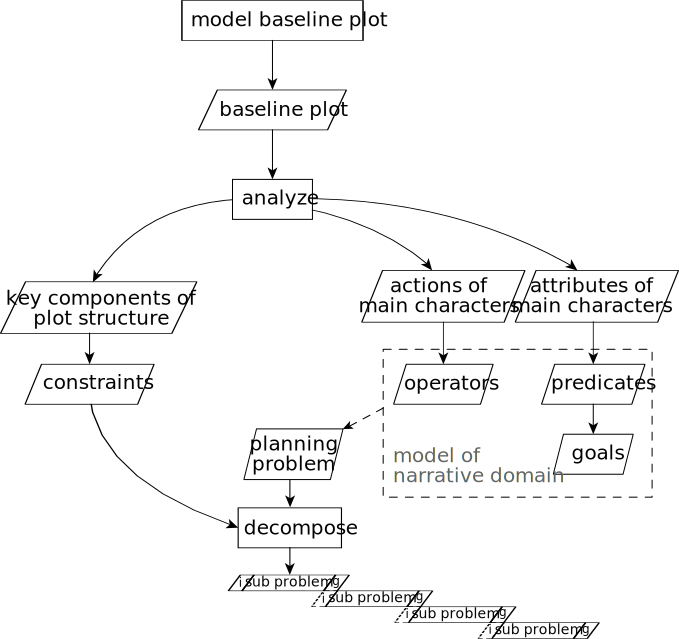
\includegraphics[scale=0.6]{discourse_model}
 \caption{Visualization of the modeling process.}
 \label{fig:modproc}
\end{figure}
\subsubsection{Planning}
